%  %% LyX 2.3.1 created this file.  For more info, see http://www.lyx.org/.
%  %% Do not edit unless you really know what you are doing.
%  \documentclass[twocolumn,english,showpacs,preprintnumbers,amsmath,amssymb,floatfix]{revtex4-1}
%  \usepackage[T1]{fontenc}
%  \usepackage[latin9]{inputenc}
%  \setcounter{secnumdepth}{3}
%  \usepackage{color}
%  \usepackage{babel}
%  \usepackage{graphicx}
%  \usepackage{esint}
%  \usepackage[unicode=true,
%   bookmarks=false,
%   breaklinks=false,pdfborder={0 0 1},backref=section,colorlinks=false]
%   {hyperref}
%  
%  \makeatletter
%  %%%%%%%%%%%%%%%%%%%%%%%%%%%%%% User specified LaTeX commands.
%  \hyphenpenalty=10000
%  
%  \makeatother
%  
%  \begin{document}
%  
\clearpage
\newcommand{\xsec}[1]{\vskip 6pt \noindent {\bf #1} \quad }

\appendix

{\small
\textbf{\textcolor{blue}{TO DO LIST:}}
\textcolor{blue}{{*} Follow up on John Collins' list {[}MOSTLY DONE{]} }
\textcolor{blue}{{*} Add brief mention at end that this applies also
to bottom quark {[}at end{]}}
\textcolor{blue}{{*} refs from Sasha: LHC W+c measurements:
  \cite{Chatrchyan:2013uja,Aad:2014xca,Sirunyan:2018hde}}
  }

\section{$F_{2}^{charm}$ Beyond Leading-Order}

\begin{figure}
\centering 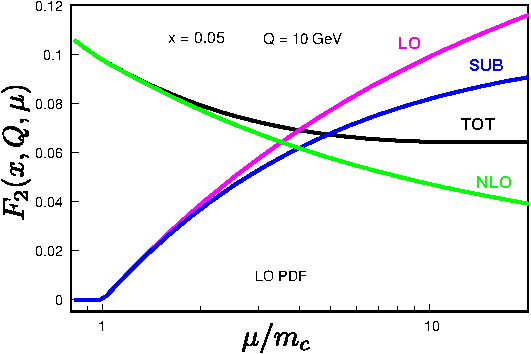
\includegraphics[clip,width=0.45\textwidth]{pics/fred/acot_fig}
\caption{Calculation of $F_{2}^{c}$ vs.\ $\mu$ in the VFNS illustrating the
cancellation of the LO ($\bar{c}W^{+}\to\bar{s}$) and the SUB \hbox{$(g\to \bar{c})$}$\otimes$\hbox{$(\bar{c}W^+ \to \bar{s})$}
contributions in the region $\mu\sim m_{c}$. The $Q$ scale is fixed
at $10\,$GeV and the charm PDF is matched at $\mu_{c}=m_{c}$ such
that $f_{c}(x,\mu=m_{c})=0$. \label{fig:acot}}
\end{figure}

\begin{figure*}
\centering 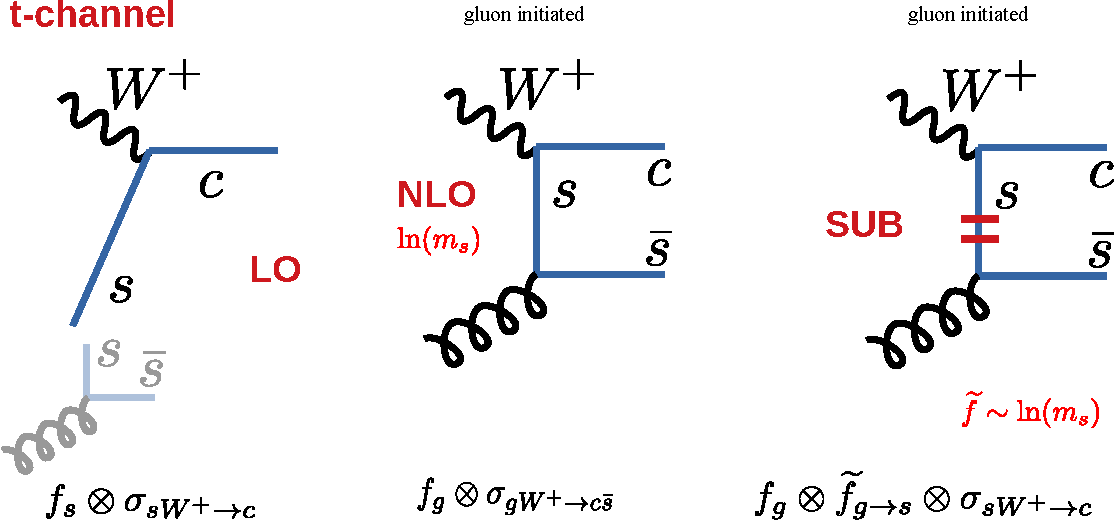
\includegraphics[clip,width=0.8\textwidth]{pics/fred/tchannel}
\caption{Gluon $t$-channel processes up to ${\cal  O}(\alpha_S^1)$.  \label{fig:tchannel}}
\end{figure*}

\begin{figure*}
\centering 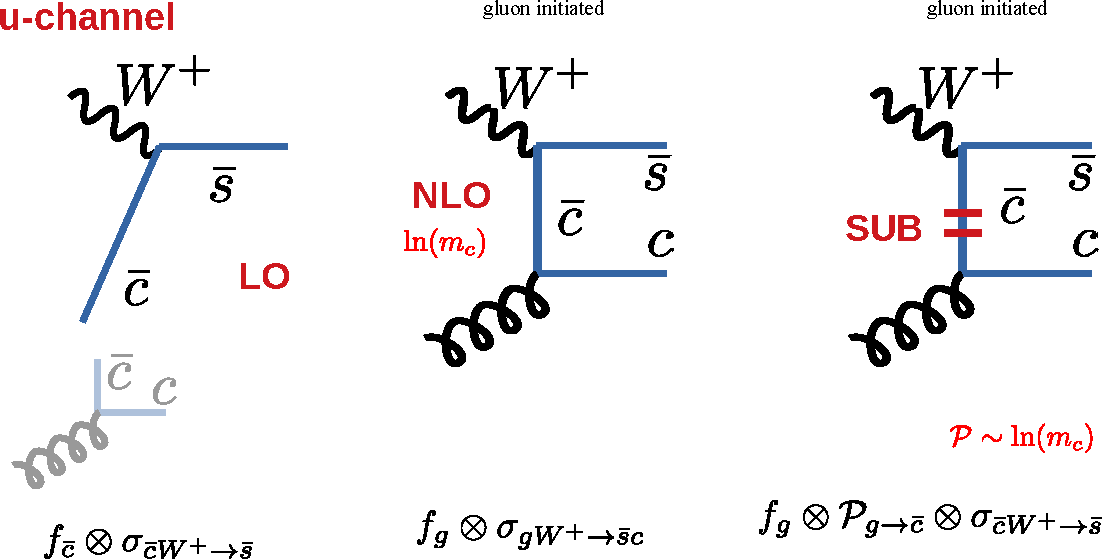
\includegraphics[clip,width=0.8\textwidth]{pics/fred/uchannel}
\caption{Gluon NLO $u$-channel processes  up to ${\cal  O}(\alpha_S^1)$. \label{fig:uchannel}}
\end{figure*}




\xsec{The Multi-Scale Problem:}
%
The charged current DIS charm production process involves some interesting
issues that we will explore here in detail. In particular, there are
multiple mass and energy scales which span a wide kinematic range,
and it becomes an intricate puzzle to treat them all properly. 

For this current illustration, we will focus on the contribution to
the DIS $F_{2}^{c}$ structure function from the process involving
the strange and charm quark; other quark combinations can be addressed
in a similar manner.
%
The  fully inclusive $F_2(x,Q^2)$ can be studied using the energy and angle of the
outgoing lepton; in contrast, $F_{2}^{c}$ also requires information about
the final hadronic state, and this introduces some subtleties.
%
In particular, we will show that as we go to
higher-orders the $F_{2}^{c}$ structure function must be defined
carefully so that i) theoretically it is free of divergences and independent
of the renormalization scales, and ii) experimentally it matches what
is measured by the detector.
%



\xsec{Overview:}
%

\textcolor{blue}{... to be filled in ... (what other detailed are needed???)}

\xsec{The Mass Scales:}
%
What makes this process complex is
that we encounter a number of different mass scales.
Furthermore, 
there is no fixed hierarchy for
the mass scales, and we will need to compute both in the low $Q$
region where $Q\lesssim m_{c}$ as well as the high $Q$ region $Q\gg m_{c}$. 

The $Q$ scale is the invariant mass of the virtual boson probe ($W^{+}$
in this case), and can be related to the energy and angle of lepton;
this is a physically measurable kinematic variable. 

In contrast, the renormalization scale $\mu$ is an unphysical scale
which implements the separation between the PDF and the hard scattering cross section; thus,
the physics should be insensitive to a variation of $\mu$. As our
calculations typically involve the dimensionless combination $\ln(\mu^{2}/Q^{2})$,
we generally choose $\mu\sim Q$ avoid large logarithms. 

The strange quark is a ``light'' active parton with an associated
PDF $s(x)$ and mass $m_{s} < \Lambda_{QCD}$. The strange quark mass is comparable
or less than other hadronic scales which are neglected; as such, it
serves only as a regulator and plays no physical role, and we can
take $m_{s}\to0$ if we choose.
%
We treat the up and down quarks masses  $m_{u,d}$ in a similar manner.

The charm quark is a ``heavy'' object; its associated mass $m_{c}> \Lambda_{QCD}$
does play a physical role and cannot be neglected. There may or may
not be a PDF associated with the charm. In a 3-flavor FFNS scheme,
we will assume the charm PDF to be zero.\footnote{It is possible to extend this to  incorporate an intrinsic charm PDF.}
In a 4-flavor VFNS there is a charm PDF only
when the $\mu$ scale is above the scale where the charm PDF is activated;
we call this the matching scale, $\mu_{c}$.
It is common\footnote{%
The choice of matching scale $\mu_{c}=m_{c}$ is common because at
NLO the $\overline{MS}$ matching conditions on the PDFs are proportional
to the DGLAP kernel times $\ln(\mu/m_{c})$, as explicit calculation
shows the constant term vanishes; thus we have the simple boundary
condition $f_{c}(x,\mu=m_{c})=0$. At NNLO, the constant term is non-zero
and this yields $f_{c}(x,\mu=m_{c})\not=0$. See \cite{Stavreva:2012bs}
and references therein.}
%5
to set $\mu_{c}=m_{c}$, but this is not
required.\footnote{%
By displacing the matching scale to larger values $\mu_{c}\gg m_{c}$,
can have the advantage of avoiding delicate cancellations in the region
$\mu\sim m_{c}$; this flexibility was explored in Refs.~\cite{Bertone:2017ehk,Bertone:2018ids}
.}
%
In this study we will fix the matching scale to this common choice:
$\mu_{c}=m_{c}$.


Because there are two different quark masses $\{m_{s},m_{c}\}$ involved
in the charged current DIS flavor-changing process,  we can examine
the mass singularities of the $t$-channel and $u$-channel separately.
%
This separation is particularly useful to understand how the individual
mass singularities are addressed, and how FFNS and VFNS organize the
contributions to the total structure function. 

\xsec{3-Flavor FFNS:}
%
To be specific, we will consider charged-current DIS production of
a charm quark. We first compute this in a 3-flavor (FFNS) scheme where
$\{u,d,s\}$ are light ``active'' partons in the proton, and charm
$\{c\}$ is considered an external ``heavy'' particle. This can
be implemented in the ACOT scheme\cite{Aivazis:1993pi} for example
by using a CWZ renormalization\cite{Collins:1978wz} where the light
``active'' partons are renormalized with normal $\overline{MS}$,
and the ``heavy'' quarks use a zero-momentum subtraction. In this
scheme, the \textbf{leading-order} (LO) process is \mbox{$sW^{+}\to c$}
as illustrated in Fig.\,\ref{fig:acot}. At \textbf{next-to-leading-order}
(NLO), we then include \mbox{$gW^{+}\to c\bar{s}$} which has both $t$-channel
and $u$-channel contributions.\footnote{Note, there are also corresponding quark-initiated processes; we will
focus on the gluon-initiated processes as this is sufficient to illustrate
our points. Both the gluon- and quark-initiated contributions are
included in our calculations. }

\xsec{$t$-Channel:}
%
The $t$-channel process has an intermediate $s$-quark exchanged, and
if we use the strange quark mass $m_{s}$ to regulate the singularities,
this will yield a contribution proportional to $\ln(Q/m_{s})$. This
mass singularity arises from the region of phase space where the exchanged
$s$-quark becomes collinear and close to the mass-shell; that is,
when the phase space of the \mbox{$gW^{+}\to c\bar{s}$} process begins to
overlap with that of the \mbox{$sW^{+}\to c$} process. This ``double counting''
is resolved by a \textbf{subtraction} (SUB) counter-term
%(which is formally part of the NLO contribution)
given by:
\[
(SUB)\sim f_{g}\otimes\widetilde{f}{}_{g\to s}\otimes\sigma_{sW^{+}\to c}\quad.
\]
Here, $\widetilde{f}{}_{g\to s}$ is the perturbative splitting of
the gluon into an $s\bar{s}$ pair; the leading term is proportional
to:\footnote{The scale of the SUB term is $\mu$ as the relevant scale here is
the renormalization scale of the PDF:$f(x,\mu)\otimes\hat{\sigma}(x,Q,\mu)$. }
\[
\widetilde{f}_{g\to s}(x,\mu)\sim\frac{\alpha_{S}(\mu)}{2\pi}P_{g\to s}^{(1)}(x)\:\ln\left(\frac{\mu^{2}}{m_{s}^{2}}\right)+\text{{\cal O}}(\alpha_{s}^{2})
\]
 where $P_{g\to s}^{(1)}(x)$ is the $\alpha_{S}^{1}$ DGLAP splitting
kernel for \hbox{$g\to s$}.

The complete contribution to the structure function is given by:
\[
F_{2}^{c}\sim TOT=LO+(NLO-SUB)
\]
The complete ${\cal O}(\alpha_{s}^{1})$ contribution is the combination
$(NLO-SUB)$; our separation into $NLO$ and $SUB$ is simply to illustrate
the interplay of these components. Both the NLO and SUB terms have
$\ln(m_{s})$ divergences, but these precisely cancel and yield a
well defined result even as we take the $m_{s}\to0$ limit.\footnote{In fact, we could have taken $m_{s}=0$ initially and used dimensional
regularization to compute the contributions.}

\xsec{$u$-Channel:}
%
We next examine the $u$-channel NLO contribution to the \mbox{$gW^{+}\to c\bar{s}$}
process. This has an intermediate $c$-quark exchanged, and is proportional
to $\ln(Q/m_{c})$. In the FFNS where the charm is a ``heavy'' non-parton,
there is no counter-term for this graph, and the resulting observables
will retain the $\ln(Q/m_{c})$ dependence. In principle, this means
when we go to large $Q$-scales, these terms will begin to degrade
the convergence of our perturbation series. In practice, while this
degradation only grows logarithmically, at large scales (such as at
the LHC) we do find it convenient to treat the charm on an equal-footing
as the ${u,d,s}$ partons. 

\xsec{4-Flavor VFNS:}
%
We now turn to the 4-flavor (VFNS) scheme where we include the charm
quark as an ``active'' parton and compute its associated PDF.

In this case, there is a $u$-channel counter-term (SUB) given by $f_{g}\otimes\widetilde{f}{}_{g\to\bar{c}}\otimes\sigma_{\bar{c}W^{+}\to\bar{s}}$
which is proportional to $\ln(\mu/m_{c})$. The NLO $u$-channel contribution
will have a $\ln(Q/m_{c})$ contribution, so the combination $(NLO-SUB)$
is also free of mass singularities.\footnote{Specifically, the combination $(NLO-SUB)$ is free of mass singularities
and finite in the limit $m_{c}\to0$. Note, the VFNS fully retains
the charm quark mass $m_{c}$ and (in contrast to some claims in the
literature) the factorization holds up to ${\cal O}(\Lambda^{2}/Q^{2})$
corrections; all terms of order $(m_{c}^{2}/Q^{2})$ are fully included.\cite{Collins:1998rz}}

What is less obvious is that we also must include the LO process \mbox{$\bar{c}W^{+}\to\bar{s}$}.
There are two ways we can understand why this is necessary. 

\xsec{Explanation \#1: Matching of LO and SUB:}
%
Recall that in the $t$-channel case, the subtraction term SUB removed
the double counting between the LO \mbox{$sW^{+}\to c$} and NLO \mbox{$gW^{+}\to c\bar{s}$}
processes. 

The $u$-channel case is analogous in that this subtraction term removes
the double counting between the LO \mbox{$\bar{c}W^{+}\to\bar{s}$} and NLO
\mbox{$gW^{+}\to c\bar{s}$} processes; both contributions are required to
ensure the resulting cross section is insensitive to the $\mu$-scale. 

This is apparent in Fig.~\ref{fig:acot} where we plot the individual
terms versus the $\mu$ scale for a fixed $x$ and $Q$. In the region
of $\mu\sim m_{c}$, the charm PDF $f_{c}(x,\mu)$ (and hence, the
LO contribution) rises very quickly as the DGLAP evolution is driven
by the very large gluon via $g\to c\bar{c}$ splitting, and combined
with a large $\alpha_{S}(\mu)$. The SUB subtraction also rises quickly
as this is driven by the logarithmic term $\ln(\mu^{2}/m_{c}^{2})$.
The difference \mbox{$(LO-SUB)$} is the physical contribution to the total
\mbox{$[TOT=LO+NLO-SUB]$}, and it is this combination which is smooth across
the ``turn on'' of the charm PDF at the matching scale $\mu_{c}=m_{c}$.
We now see that if we neglect the LO \mbox{($\bar{c}W^{+}\to\bar{s}$)} contribution,
we lose the cancellation between LO and SUB in the region $\mu\sim m_{c}$,
and our structure function (or cross section) would have an anomalous
shift at the arbitrarily location $(\mu_{c})$ where we turn on the
charm PDF. 

As we vary the unphysical renormalization scale $\mu$, we are simply
shifting contributions between the separate \mbox{$\{LO,NLO,SUB\}$} terms
which individually exhibit a large $\mu$-dependence. However, the
total combination $(TOT)$ which represents the physical observable
is relatively insensitive to $\mu$ (up to higher orders), and this
property is evident in Fig.~\ref{fig:acot}.

\xsec{Explanation \#2: Removing ``Double Counting:''}
%
A second way to understand why we require the LO process \mbox{$\bar{c}W^{+}\to\bar{s}$}
is to consider the regions of phase space covered by each of the sub-processes.
The singularity of the $u$-channel NLO \mbox{$gW^{+}\to c\bar{s}$} processes
arises the phase space region when the intermediate $\bar{c}$ quark
becomes collinear and close to the mass-shell.\footnote{Specifically, the charm quark is off-shell by the order of its mass
$m_{c}$; this is independent of the scale $Q$ and \textbf{\textit{does
not}} assume any $Q\gg m_{c}$ limit. } This is precisely the phase space region of the LO process \mbox{$\bar{c}W^{+}\to\bar{s}$}
where the partonic $\bar{c}$-quark is collinear to the hadron. The
SUB term then removes the ``double counting'' between the LO and
NLO contributions; hence, all three contributions \mbox{$\{LO,NLO,SUB\}$}
are necessary to cover the full phase space.

This is also apparent if we consider the transverse momentum $(p_{T})$
of the final-state charm in the Breit frame. For the LO \mbox{$\bar{c}W^{+}\to\bar{s}$}
process in the Breit frame, the incoming $W^{+}$ and $\bar{c}$ are
collinear, and the produced $\bar{s}$ must have zero $p_{T}$ in
this frame.

For the NLO $gW^{+}\to c\bar{s}$ process, we integrate over the complete
phase space for the exchanged $\bar{c}$ quark, and this will include
the region where the $\bar{c}$ quark is emitted nearly collinear
to the gluon and nearly on-shell; in this region the $\bar{c}$ quark
will have $p_{T}\sim0$ and we encounter a singularity from the internal
$\bar{c}$ propagator. The $p_{T}\sim0$ region is precisely that
subtracted by the SUB counter term,\footnote{Specifically, the incoming $W^{+}$ and $g$ are collinear, and the
gluon then emits a collinear $c\bar{c}$ pair so the final $\bar{s}$
has zero $p_{T}$.} and this ensure that the combination $(NLO-SUB)$ is free of divergences.



\xsec{Recap:}
%
To recap, i) the combination of the LO and SUB terms ensure a minimal
$\mu$-variation at low $\mu$ scales, and ii) the combination of
SUB and NLO ensure the mass singularities are canceled at high $\mu$
scales.

This interplay of the terms illustrates some of the intricacies of
QCD, especially since this exchange is across different orders of
$\alpha_{s}$.


Furthermore, note that in the $u$-channel for both the LO and SUB contributions,
the charm quark is collinear with the incoming hadron, and thus exits
in the hadron remnants. While this may be experimentally difficult to observe,
because we are asking for a \textit{``fully inclusive''} $F_{2}^{c}$,
these contributions cannot be simply ignored. We will discuss this
further in the following section. 

\xsec{Defining $F_{2}^{c}$:}
%
The $u$-channel LO \mbox{$\bar{c}W^{+}\to\bar{s}$} process foreshadows difficulties
we encounter if we try and extend the concept of a ``fully inclusive''
$F_{2}^{c}$ to higher orders. We note that in Ref.~\cite{Collins:1998rz}
Collins extended the proof of factorization to include heavy quarks
such as charm and bottom for an inclusive structure function $F_{2}$;
there is no corresponding proof for an \textit{``fully inclusive''}
$F_{2}^{c}$.
%
Whereas $F_2(x,Q^2)$ only requires measurement  of the outgoing lepton
energy and angle,  $F_2^c(x,Q^2)$ also requires information of
the final state.
At the parton-level this introduces complications
including when the charm is in the hadronic remnants, and brings in
both fragmentation functions and fracture functions.

To characterize the theoretical issues involved in constructing 
$F_{2}^{c}$, we can imagine starting from the (well defined) inclusive
$F_{2}$, and then dividing the contributions into two sets: one for
$F_{2}^{c}$ for the ``heavy'' charm quark, and the rest into $F_{2}^{u,d,s}$
for the ``light'' quarks. We will show this theoretical procedure
encounters ambiguities.

The $u$-channel LO $\bar{c}W^{+}\to\bar{s}$ process does not have any
``apparent'' charm quark in the final state, but this contribution
is essential to balance with the SUB process
\mbox{$f_{g}\otimes\widetilde{f}{}_{g\to\bar{c}}\otimes\sigma_{\bar{c}W^{+}\to\bar{s}}$.}
Note that for the SUB process, the charm quark arises from a gluon
splitting into a collinear $c\bar{c}$ pair which is then part of
the hadron remnants. For the LO process, presumably our $\bar{c}$
quark also came from a gluon splitting into a collinear $c\bar{c}$
pair. Thus, our $F_{2}^{c}$ must include those cases where the charm
in contained in the hadron remnants.

This issues touches on the fact that because the charm parton
ultimately fragments into a  charm meson (typically a
$D^{*}$) via a fragmentation process we must  introduction
of a set of fragmentation functions (FFs) which are scale-dependent
and will factorize final-state singularities in a similar manner as
the PDFs factor the initial-state singularities.\footnote{Also note, for the NLO quark-initiated contributions (not shown) we
will have final state singularities from processes such as $c\to cg$
which will be factorized into the fragmentation functions.}
Note we also must allow for the possibility that a gluon or light quark
can also produce a charm meson. 


\xsec{The Bubble  Diagram:}
%
\begin{figure}[t]
\centering 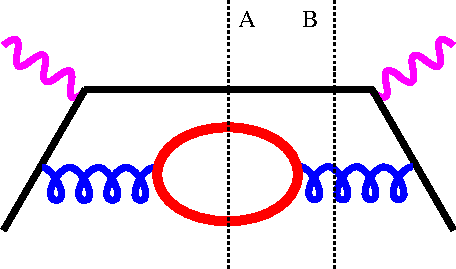
\includegraphics[width=0.45\textwidth]{pics/fred/feyngraph}
\caption{A higher order Feynman graph illustrating the complications in defining
  a ``fully inclusive'' $F_{2}^{charm}$.
 A light quark ($q$)
 scatters from a vector boson ($V$) with 
 a $c\bar{c}$ in the internal loop.
 If we cut the amplitude at  ``A''
we have charm in the final state and this must be included in $F_{2}^{charm}$.
If we cut the amplitude with cut ``B'' there is no charm in the
final state.
Additionally, since this diagram contributes to the beta function,
this highlights the complications of using an $\alpha_{S}$ and hard
scattering $\hat{\sigma}$ with differing $N_{\rm eff}$. \label{fig:bubble}}
\end{figure}

Some of the theoretical intricacies of  defining a \textit{``fully inclusive''} $F_{2}^{c}$
are illustrated in Fig.~\ref{fig:bubble} which shows
a higher-order DIS process with a quark--anti-quark loop.

Let us
compute this diagram in a 3-flavor FFNS where the internal loop is
a $c\bar{c}$-pair, and the external quark is a light \mbox{$\{u,d,s\}$}.
If the final-state is represented by Cut-A, then we have charm quarks
in the final state, and this should be included in $F_{2}^{c}$. 

However, if we instead use Cut-B as the final state, there is no charm
in the final state, so this should not be included in $F_{2}^{c}$.
[More precisely, when we renormalize the charm loop with zero-momentum
subtraction, this contribution effectively decouples.] Thus, the
contribution from Cut-A will be included in $F_{2}^{c}$, but the
contribution from Cut-B will not.

This diagram generates additional complications  in that multiple quark
favors are involved.
For example, the bubble diagram involves quarks of both $q$ and $c$ flavors,
so this contribution cannot be uniquely assigned to  $F_{2}^{q}$ or  $F_{2}^{c}$.
We can introduce theoretical definitions to make the choice, but
then we have to be careful about double-counting contributions and introducing
uncancelled singularities. 
%
For example, the bubble diagram of Fig.~\ref{fig:bubble} is encountered
in the $F_{2}^{c}$ heavy quark calculations of Refs.~\cite{Chuvakin:1999nx,Chuvakin:2000jm};
here, an additional scale $\Delta$ is introduced to subdivide the contributions. 



\xsec{The running $\alpha_{S}$ in the FFNS:}
%
The bubble diagram of Fig.~\ref{fig:bubble} also highlights the
difficulty of using a $N_{\rm eff}=3$ FFNS with an $N_{\rm eff}=4$ flavor
running $\alpha_{S}(\mu)$. In a $N_{\rm eff}=3$ FFNS, internal $c\bar{c}$
loops decouple from the theory and are not included in the calculation;\footnote{%
More precisely, the heavy quarks are renormalized with zero-mass-subtraction
and their contributions decouple; this is why we can neglect loops from the the top quark
and any other heavy particle.
}
%
however, the $N_{\rm eff}=4$ $\beta$-function requires precisely these
$c\bar{c}$ loop contributions.\footnote{Note; this deficiency can in principle be patched order-by-order by
expanding the $\beta$-function and inserting the required terms at
each order~\cite{Napoletano:2014thesis,Bierenbaum:2009zt,Cascioli:2013era}. }
Once again, we cannot unambiguously divide the inclusive $F_{2}$
into separate ``light'' and ``heavy'' quantities. 



\xsec{Extensions to bottom and top:}
%
While we have used the charm quark to illustrate these features, the
same properties can, in principle, be applied to both the bottom and
top quark.\footnote{Additionally, Collins specifically addressed the case of multiple
heavy quarks which can allow for both charm and bottom in a unified
framework; in contrast to some incorrect claims in the literature,
there is no difficulty including multiple heavy quarks. (C.f, Ref.~\cite{Collins:1998rz},
Sec.~IX.)} For the case of the bottom quark, the larger mass $m_{b}$ yields
a smaller $\alpha_{s}(\mu)$ for $\mu\sim m_{b}$ and the evolution
of $f_{b}(x,\mu)$ is thus reduced; nevertheless, for large scale
processes (such as the LHC) we often find it convenient to make use
of $f_{b}(x,\mu)$ and treat the 5-flavors on an equal footing. 
%
For the case of the top quark, the very large
mass $m_{t}$ yields a much smaller $\alpha_{s}(\mu)$  for $\mu\sim m_{t}$  and the evolution
of $f_{t}(x,\mu)$ is comparatively reduced.




\subsection*{Summary }

To properly define an $F_{2}^{c}$ at higher-orders, we encounter the theoretical issues
discussed in the above; as fragment the charm quark to the charm meson and,
and  we must be careful to ensure the  theoretical quantity to what is actually measured experimentally.
*** NOT UPDATED YET HERE ***
{\it This is more complex than simply asking for the portion of $F_{2}$
which has charm in the final state, and is an issue for both the FFNS
and VFNS. The experimental $F_{2}^{c}$ is a differential cross section
for producing a charm meson in a fiducial region; this physical observable
is singularity-free and $\mu$-independent. }

We can compute in the FFNS, but in the large energy limit, we encounter
$\ln(Q^{2}/m_{c}^{2})$ divergences and this, in part, contributes
to the observed differences at large $Q$ scales. 

The VFNS includes the charm quark as an active parton for $\mu$ scales
above a matching scale $\mu_{c}$. For large $Q$ scales, the mass
singularities of NLO and SUB will cancel to yield a result free of
divergences. For scales $\mu\sim m_{c}$, cancellation between the
LO and SUB contributions ensures minimal $\mu$ dependence; however,
as this can be delicate to implement numerically, we have the option
of displacing the matching scale $\mu_{c}$ to a larger scale where
the cancellation is more stable.\cite{Bertone:2017ehk,Bertone:2018ids}


%\subsection*{Acknowledgements}
%Thanks to:
%John Collins, Ted Rogers, George Sterman, Ingo Schienbein, Aleksander Kusina

%\bibliographystyle{unsrt}
%\bibliography{fred}

%\end{document}
